\chapter{The Last Bulk Optics Experiment}
\label{ch:BulkCircuit}

\section{Introduction}
In this chapter, I describe the calibration and testing of a completely
reconfigurable circuit in bulk optics. By altering the parameters in this single
experiment, we were able to simulate the action of any lossless linear optics
circuit on four modes. The architecture was motivated by (but not identical to)
the scheme described by Reck et al in \cite{reck94}. An application of this
circuit to quantum simulation is described in chapter~\ref{ch:Simulations}.

\begin{figure}
  \centering
  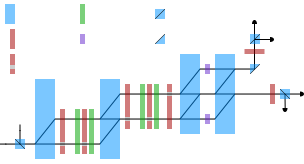
\includegraphics{scatterbox/calibration/figures/circuit.pdf}
  \caption{A schematic of the bulk optics circuit. Two photons are injected at
the left of the circuit in orthogonal polarisations (\(\ket{H}\) indicates
horizontal and \(\ket{V}\) indicates vertical), using an in-fibre polarising
beamsplitter
(PBS) to combine the two photons into a single path. The circuit operates in a
combined path/polarisation encoding, where polarising beam displacers (PBD) are
used to convert between the two. Operations are performed with fixed quarter
waveplates (QWP) and polarisation flips (X), and variable angle half waveplates
(HWP). After the operations are complete, polarisation-sensitive detection is
performed using further PBS elements and single photon avalanche diodes. We
label the detectors A through D.}
  \label{fig:circuit}
\end{figure}

\section{Calibration (the crapusoids are real)}

\begin{figure}
  \centering
  \begin{subfigure}{\textwidth}
    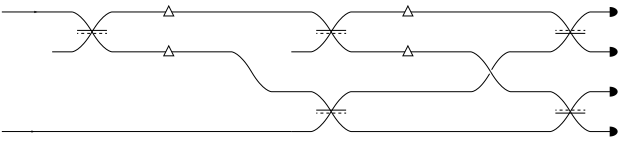
\includegraphics{scatterbox/calibration/figures/schematic.pdf}
    \caption{A schematic of the circuit, expanded into path}
    \label{fig:schematic}
  \end{subfigure} \\
  \vspace{1cm}
  \begin{subfigure}{0.45\textwidth}
    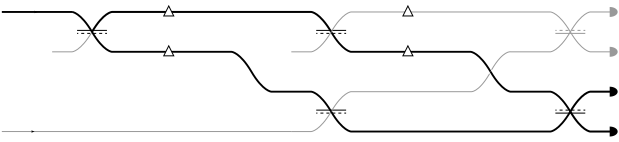
\includegraphics{scatterbox/calibration/figures/interferometerAB.pdf}
    \caption{A/B interferometer}
    \label{fig:ab}
  \end{subfigure}
  \hspace{0.05\textwidth}
  \begin{subfigure}{0.45\textwidth}
    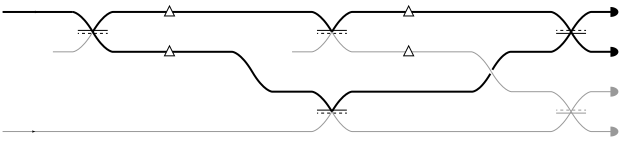
\includegraphics{scatterbox/calibration/figures/interferometerCD.pdf}
    \caption{C/D interferometer}
    \label{fig:cd}
  \end{subfigure}
  \caption{Interferometers}
  \label{fig:interferometers}
\end{figure}

\section{Benchmarking (arguably the first boson sampler)}
